\chapter{Technical Implementation}
\label{sec:technical_implementation}
This section covers the technical part of the pipeline. There will not be much discussion about 
whether one of the pipeline is better than the other or if the implementation is good or not.
Rather I will reflect and discuss that in 
the discussion section \ref{sec:discussion-pipeline}.
Section \ref{sec:pipeline_remote} is about the remote deployment.
Section \ref{sec:pipeline-local} is about the final pipeline product hence 
the local pipeline and it's local deployment.\\\\
The objective of this pipeline is to provide developers with an environment where they can develop and experiment, 
using a setup akin to the production pipeline. They have the flexibility to integrate their own repositories, 
configurations, and other resources into the pipeline to observe its behavior. This enables them to assess and 
refine their development practices based on the pipeline's performance.

Localized pipelines, although less common nowadays, offer a unique advantage. Unlike pipelines hosted on 
cloud-based virtual environments managed by service providers, a localized pipeline resides directly on the developer's machine. 
This grants developers full access to the pipeline's infrastructure, codebase, and configurations. Such accessibility is invaluable 
considering the prevalent use of pipelines 
in modern development workflows, emphasizing the importance of adhering to secure and efficient practices.
For this project the pipeline is constructed with the components that are described in section \ref{sec:tools}.


\section{Pipeline - Remote}
\label{sec:pipeline_remote}
For the first part of the project there was a major a problem with authenticating user between the Gitea server and 
the Drone server.\\
This problem was solved by using a remote Gitea instance which could be accessed over the internet. This meant that the 
Gitea server would not be run locally on a users machine, but instead on a remote server. The Drone server, Drone runners and everything 
related to the deployment of Drone with be on the users end, hence using the users resources. This is how that deployment worked. It consisted of 
five parts:

\begin{itemize}
    \item Gitea configuration (Docker)
    \item Drone configuration (Docker)
    \item Admin (Python script)
    \item Webhook (Python script)
    \item Request script (Python script)
\end{itemize}
This solution for a pipeline had drawbacks, but that will be discussed in the section \ref{sec:discussion-pipeline}. Here
the sole focus is on how the 
product worked and how it was implemented.

\subsection{Gitea configuration}
The Gitea configuration was first created with the intention of being run locally. However, because of the Oauth2 authenticating problem, 
the Gitea server was moved to a remote server. This meant that, although it was possible to close, delete, and recreate the Gitea server with the same configuration, it was no longer necessary. 
However, this configuration made it easy to restart the server if needed.
For the deployment of the Gitea server, the following command was used:
\begin{figure}
    \begin{center}
        \centering
        \javaf{docker compose up -d}
        \caption{Docker compose command use for remote Gitea}
        \label{fig:docker-compose-remote}
    \end{center}
\end{figure}
The command showed in figure \ref{fig:docker-compose-remote} is the basic command for running Docker compose detached. 
Now behind that command is the docker-compose.yml\cite{docker-compose} file.
The docker-compose.yml file is used to define the configuration of the Gitea server. The file is shown below:
\begin{figure}[h]
    \begin{lstlisting}[style=yaml]
        version: '3'
        networks:
            kv:
                name: kv
                driver: bridge
        services:
            gitea:
                image: kraftvaerket/kv-gitea:latest
                container_name: Gitea
                restart: always
                environment:
                    - USER_UID=1000
                    - USER_GID=1000
                networks:
                    - kv
                ports:
                    - "3000:3000"
    \end{lstlisting}
\caption{docker-compose.yaml file for Gitea}
\label{sec:pipeline_remote_gitea_docker_compose}    
\end{figure}

\begin{itemize}
    \item \textbf{image}: Specifies the Docker image to use for this service, in this case, "kraftvaerket/kv-gitea:latest".
    \item \textbf{container\_name}: Specifies the name of the container, in this case, "Gitea".
    \item \textbf{restart}: Specifies the restart policy for the container, in this case, "always", which means Docker will always restart the container if it stops, regardless of the exit status.
    \item \textbf{environment}: Specifies environment variables to be passed to the container. Here, it sets the user UID and GID to 1000.
    \item \textbf{networks}: Specifies which networks this service should be connected to. In this case, it'sconnected to the "kv" network.
    \item \textbf{ports}: Specifies port mappings between the container and the host. In this case, it maps port 3000 on the host to port 3000 on the container, allowing access to the Gitea application running inside the container.
\end{itemize}
The overall of this docker-compose file is simple and basic since all of the configurations were done in the image itself.
The image used is a custom image created by the author, which 
is pulled from DockerHub. Doing all the configurations 
in the image, creates a more robust image that is more reliant to work on different machines.

This Docker compose file was then run on a \ac{Ucloud} machine which then created the Gitea server. 
To make the Gitea server accessible from the internet with another \ac{URL} than \\
\javaf{http://localhost:3000}, a reverse proxy was used called Ngrok \cite{ngrok}.
Ngrok is attached to the Gitea server by running the software running along side the Gitea server.
For that to be done you need to run the following command:
\begin{figure}[h]
    \begin{center}
        \javaf{ngrok http 3000 https://full-enormous-crow.ngrok-free.app}
    \end{center}
    \caption{Ngrok command}
    \label{fig:ngrok-command} 
\end{figure}

\begin{itemize}
    \item
    \javaf{ngrok}\\Ngrok CLI \\
    \item 
    \javaf{http 3000} \\Ngrok communicates with the Gitea server on port 3000 with the protocol http\\
    \item
    \javaf{https://full-enormous-crow.ngrok-free.app}\\Public \ac{URL} that ngrok provides
\end{itemize}

\subsection{Drone configuration}
For Drone to function, it relies on Gitea for user authentication through OAuth2. 
This means the Gitea server must be running before the Drone server can start. 
Since the Gitea server was running remotely and continuously, the Drone server could be started without any issues.

For the remote solution, it still meant that the Drone server and runners would be running locally.
The drone server is started by running a bash script, that would start the Drone server and runners.
This bash script had several functions
\begin{itemize}
    \item First:
    It checked whether all the necessary programs was installed on the machine. If not, the script would exit.
    \item Second:
    Creating a user, followed by the creation of an Oauth2 Application, for that particular user.
    The user would use these credentials to authenticate Drone with the Gitea server.
    \item Third:
    It spawned all the necessary Docker containers, both the server and the runners.
    \item Fourth:
    A newly created repository had to be activated and only after activation, it 
    was it possible to post secret and other configuration a specific repository.
    The script uses the Drone \ac{API} to activate the repository and add necessary secrets that might be used for a CTF or 
    other part of the pipeline.
    To accomplish this, the script required admin credentials for the Drone server. 
    The process involved the user logging in as an admin on the remote Gitea server, 
    authenticating as an admin on the local Drone server, and then navigating to the admin page to copy the token. 
    This token was then input into the script and used to create configurations and backend components for the Drone server.
\end{itemize}
In figure \ref{sec:pipeline_remote_drone_start_script} a snippet of the bash script is shown.
The entire script can be found in the source code under \javaf{archive/drone/drone.sh}.

\begin{figure}[h]
    \centering
    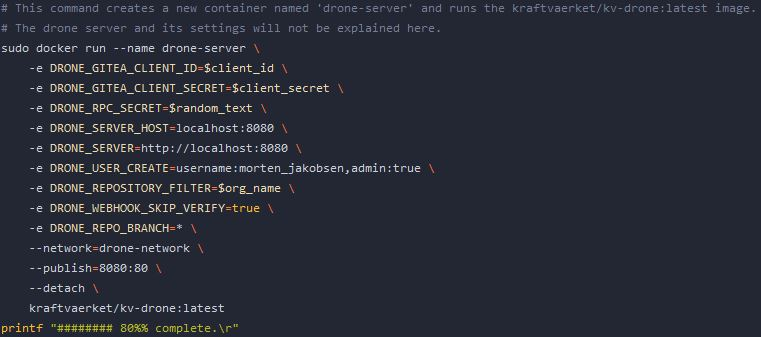
\includegraphics[scale=.69]{images/remote-script-drone.jpg}
    \caption{Drone start script snippet}
    \label{sec:pipeline_remote_drone_start_script}
\end{figure}

The image displays several environmental variables,
you see several environment variables, 
but the two most important ones are; \\ \javaf{DRONE_GITEA_CLIENT_ID} and \javaf{DRONE_GITEA_CLIENT_SECRET}. 
These variables are used to authenticate the Drone server with the Gitea server. 
While the host and RPC secrets for the Drone runners are necessary, 
the authentication credentials for OAuth2 are essential to Drone server to enable it to authenticate itself and the users 
wanting to use it.
To create the OAuth2 credentials 
on the Gitea server, a request script is utilized. This script uses the credentials provided by the user to create an OAuth2 application on the 
Gitea server for that specific user. The command in the script that executes this process is:
\begin{figure}
    \begin{center}
        \javaf{python3 ../requests/request.py $username $password}
    \end{center}
    \caption{Request script command}
    \label{fig:request-script-command}
\end{figure}
The script makes a \javaf{POST} request to the Gitea server and receives the OAuth2 credentials in return.\\
Once the pipeline was deployed and the user was created, webhooks needed to be configured. 
The purpose of the webhook is to listen for any changes in the repositories on the Gitea server. 
When a change is detected, the webhook would sends a request to the Drone server to initiate a pipeline.\\
Since the Gitea server is remote and the Drone server is local, 
an SSH tunnel is required from the remote Gitea server to the local Drone server. 
This is necessary because the Gitea server was hosted on \ac{Ucloud}, and the only way to access the machine is through SSH. 
To establish this connection, a tunnel is created from the Gitea server machine to the machine running the Drone server using the following command:\\
\begin{figure}{h}
    \begin{center}
        \javaf{ssh -Nf -L (GITEA_SERVER_MACHINES PORT):localhost:8080} \\
        \javaf{-i (SSH_KEY_FOR_LOCAL_DRONE_SERVER_MACHINE)}\\
        \javaf{USERNAME@IP_ADDRESS}
    \end{center}
    \caption{SSH tunnel command}
    \label{fig:ssh-tunnel}
\end{figure}
To establish the tunnel, the Gitea server machine needs an SSH key that can access the local machine running the Drone server. 
This is achieved by generating an SSH key on the Gitea server machine and copying the public key to the local machine.\\
Once the connection is established, a Python API on the Gitea server makes POST requests to the Drone server. 
The Gitea webhook sends a POST request to the local Flask API, which then relays the request to the Drone server.\\
\newpage

\section{Pipeline - Local configuration}
\label{sec:pipeline-local}
The localized pipeline is constructed with the components 
that are described in section \ref{sec:tools}, but the components are:

\begin{itemize}
    \item Gitea
    \item Drone
    \item Nginx
    \item Docker
    \item Local registry
    \item Certificate 
\end{itemize}
\subsection{Pipeline deployment}
\label{sec:pipeline-local-deployment}
The deployment of the pipeline is currently only available for certain operating systems. The operating systems that are supported are
\javaf{Ubuntu} and \javaf{Kali}. The deployment is done through a script \javaf{prerun.sh} that is located in the src directive of the repository.
The script consist of two parts. 
\paragraph{Part 1} of the script controls all the prerequisites that are needed for the pipeline to run. Without 
these prerequisites, the pipeline will not be able to run. The prerequisites are:
\begin{itemize}
    \item Package control. The script needs a certain number of specific packages to be installed. The packages are: \javaf{docker},
    \javaf{docker-compose}, \javaf{curl}, \javaf{python3}, \javaf{jq}, and \javaf{openssl}. There are also some packages needed that are not listed, 
    but they are preinstalled on all Ubuntu\cite{ubuntu} and Kali\cite{kali} systems.
    \item Creation of a \javaf{docker network}. This network is where all the containers will be located and communicate over.
    This network is also where the gateway to the reverse proxy is located. Without this network, the user would not be able to communicate with the pipeline.
    \item When the \javaf{docker network} is created, the script will insert a \ac{DNS} record in the 
    \javaf{/etc/hosts} file generic to Ubuntu and Kali systems. This is done so that the user can access the website with a \ac{DNS} record.
    \item Last in the first part of the script is the insertion of the certificate created for 
    the pipeline. The certificate needs to be inserted into the hosts\\
    \javaf{/etc/ssl/certs/ca-certificates.crt} file because the drone runners will use the host volumes for its certificate.
\end{itemize}
The first part of the script ensures that all prerequisites are met. The final command of part 1 initiates the spawning of containers. 
The script uses Docker Compose for this task, and the command used is shown in Figure \ref{fig:docker-compose-localized}.\\
When the first part is complete without error, the script shown in Figure \ref{fig:docker-compose-localized}.
\begin{figure}[h]
    \begin{center}
        \javaf{docker compose --env-file .env up --build -d}
    \end{center}
    \caption{docker compose command to spawn localized pipeline containers}
    \label{fig:docker-compose-localized}
\end{figure}


\paragraph{Second part} of the script waits for the containers to be up and running.
All the commands in the second part of the script is a health check to see if everything is running correctly.
It is also to make the user wait until everything works. Some of the containers depends on other containers, and 
therefore if interacted with before those containers are ready, would mean that there could be a potential error.


\subsection{Gitea}
\label{sec:pipeline-local-gitea}

When Gitea is running it must be fully configurated and ready to be interacted with.
This setup begins in the \javaf{Dockerfile.gitea}, 
where the Gitea instance is built with the necessary configurations. If Gitea does not receive an initial configuration, 
the user will encounter an initial setup page upon their first visit to Gitea, as shown in Figure \ref{fig:gitea-setup}.
\begin{figure}[h]
    \centering
    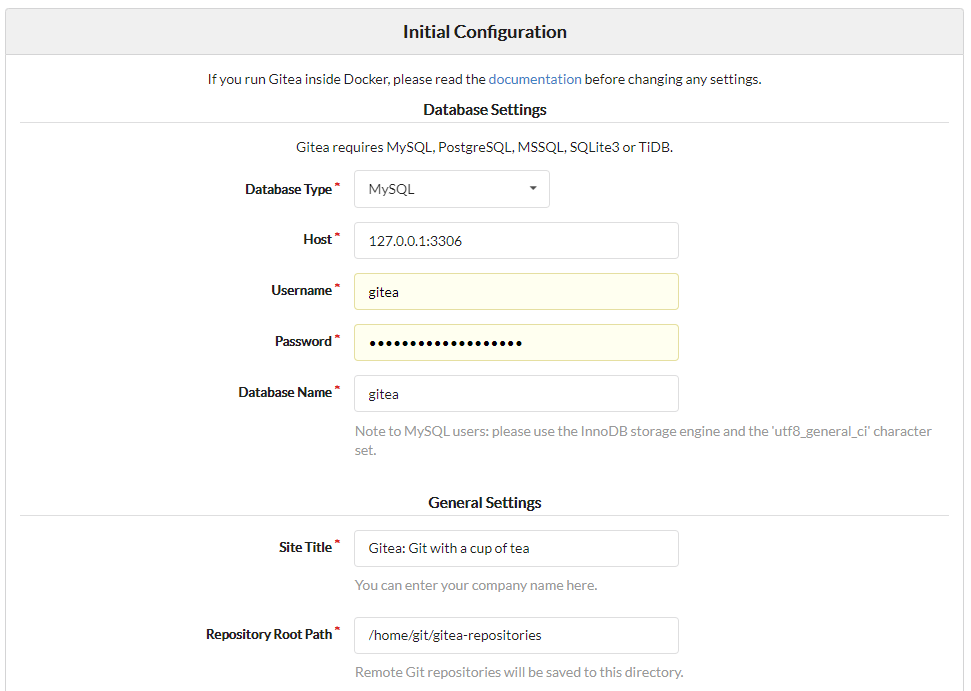
\includegraphics[width=0.8\textwidth]{images/initial_conf.png}
    \caption{Gitea setup page}
    \label{fig:gitea-setup}
\end{figure}
To avoid this, the deployment is provided with two things.

\textbf{First} is the \javaf{app.ini} file, which is the configuration file for Gitea. If no \javaf{app.ini} file is provided, 
it will be populated with data from the initial configuration page. The \javaf{app.ini} file is located in \javaf{src/gitea/config/app.ini}.

\textbf{Second} is a minimal installation of Gitea. This minimal installation is found in \javaf{src/gitea/config/gitea.tar.gz}. 
It is a simple setup of Gitea that, after the initial configuration, takes only a minute to set up. By placing the \javaf{gitea.tar.gz} file in the container 
directory \javaf{\data}, the Gitea instance will be set up with this minimal installation.
After initialization of Gitea, the script \javaf{src/gitea/start.sh} is run.
The script will curl the Gitea application to wait until Gitea is running.
The script will create \javaf{users}, \javaf{tokens}, \javaf{webhooks}, \javaf{Oauth} and \javaf{Oauth_grant}.
The script collects the information about these things from \javaf{src/gitea/config/}.

\subsection{Drone}
\label{sec:pipeline-local-drone}
Drone uses a script to initialize all the infrastructure supporting the pipeline and the underlying \ac{CTF}'s. 
Typically, when the drone is initialized, it contains no users or information about repositories. However, for a localized pipeline, 
it would be highly advantageous to have repositories and users present before the users first log in to the pipeline.

The initialization script for Drone resides in \javaf{src/drone/init.sh}. 
Since there is no direct access to the Drone data before the actual program starts through the 
\ac{API} or \ac{CLI}, a database.sql file is created, manipulated, and fed to the Drone container.
Drone utilizes a SQLite database, and data is inserted into the database using \javaf{sqlite3} commands. 
An example of a command used to insert users into the Drone database is depicted in Figure \ref{fig:sqlite3-insert}. 
The complete script can be viewed in the source code.

\begin{figure}
    \begin{center}
        \javaf{sqlite3 /data/database.sqlite "INSERT INTO users"}
    \end{center}
    \caption{sqlite3 command to insert users into the drone database}
    \label{fig:sqlite3-insert}
\end{figure}

To create and define these users and repositories before the drone program starts, 
they must match exactly on the Gitea side. 
Drone utilizes configuration files from the \javaf{src/drone/config/} 
folder to create the users and repositories. The configuration data in these \ac{CSV} files are identical to those used to create users and push repositories to Gitea.

\subsection{Nginx proxy}
\label{sec:pipeline-local-nginx}

Whenever a user interacts with the infrastructure, it will 
request by \ac{DNS} record to the gateway of the Docker Network, nginx reverse proxy, when then pickup that request, and 
proxy it to the correct container. The reverse proxy is also located inside a container, and is able through the Docker network,
to communicate with other containers. If another container outside the \javaf{docker network}
would like to communicate with a application inside the network, it would have to
go through the reverse proxy.

As described in section \ref{sec:nginx}, the reverse proxy is configuration is located in \javaf{src/proxy/default.conf}.
The conf file has three server blocks which includes the \javaf{ssl_certificate}, \javaf{ssl_conf}, and the \javaf{proxy_pass}.
These three things define what the reverse proxy does whenever a user calls the DNS record. The \ac{DNS} record for a 
specific server block is defined as \javaf{server_name}. The configuration for the proxy pass to Gitea is shown in Figure \ref{fig:nginx-proxy-pass}.

\begin{figure}[h]
    \centering
    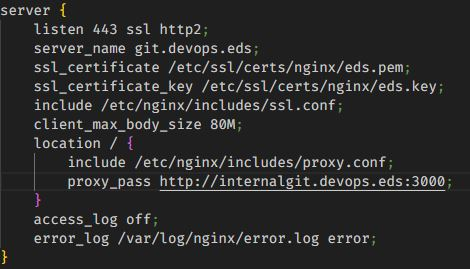
\includegraphics[scale=.7]{images/git_proxy_pass.jpg}
    \caption{Nginx proxy pass to Gitea}
    \label{fig:nginx-proxy-pass}
\end{figure}

\subsection{Docker}
\label{sec:pipeline-local-docker}
Docker serves as the backbone of the pipeline, facilitating easy deployment, maintenance, and development. 
Leveraging Docker as the containerization tool enables deployment and utilization across various environments. 
The Docker containers are specified in the \javaf{docker-compose.yml} file, located within the \javaf{src} directory.

Docker will spawn five containers and attach itself to the Docker network, when the \javaf{prerun} script is run.
\javaf{Nginx}, \javaf{Gitea}, \javaf{Drone}, \javaf{Registry}, and \javaf{Drone-runners}.
Whenever the pipeline is spawned Docker will create new images. This is to make sure that, if new changes are made 
that they are included in the new run. Docker can sometimes force itself to use cached images instead of building new 
ones if the changes are small.

The configuration for the pipeline all relies in the \javaf{docker-compose.yml} file. If any of the link, volumes, network etc. 
is wrongly configured, the pipeline might run, but it might mean that a CTF or a webhook will not create the desired outcome.\\
Differently from the remote pipeline, in the localized pipeline, Gitea and Drone are supplied with the Oauth2 application and Oauth2 grant
before it is initialized. 
By doing so, the user will not have to go through the initial setup of the application and will have access 
right away to Drone without having to authenticate through Gitea.

\subsection{Registry}
\label{sec:pipeline-local-registry}
As the project needed a local registry to fetch and push images into, the registry is a crucial part of the pipeline.
The registry used is developed by Distribution.\cite{registry}
The registry is a image registry similar to DockerHub, although DockerHub is actually isn't a registry, but a 
frontend to view available images. 
Typically, when users use the \javaf{docker pull} command, images are fetched from DockerHub. 
However, when utilizing a local registry, ensuring that images are pulled from it requires specific steps. 
The container hosting the registry must include a designated \javaf{certs} folder to inform Docker that the local registry, 
which employs a self-signed certificate, is a trusted source.\\
To establish trust in the untrusted registry mirror, the certificate must be placed in the root Docker configuration folder, specifically in \\ 
\javaf{/etc/docker/certs.d/}, with the URL of the registry, in this case, being \\
\javaf{registry.devops.eds}.
Then whenever a users or a runner wants to pull an image from the registry, it will have to use the specific URL.
see figure \ref{fig:specific_registry_url} for 
an example of a image pull in a pipeline.\\
\begin{figure}
    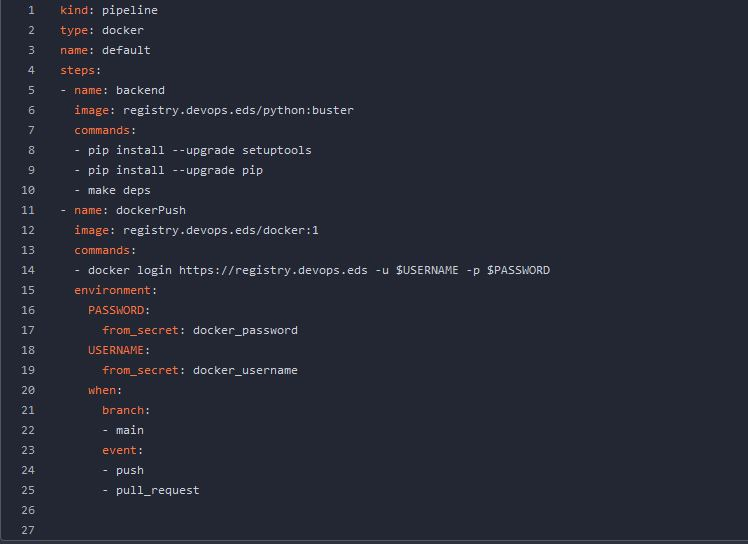
\includegraphics[scale=0.65]{images/local-registry-pull.jpg}
    \caption{Pulling an image from the local registry}
    \label{fig:specific_registry_url}
\end{figure}
The local registry work just like \url{https://registry-1.docker.io}. Although it different from \url{https://hub.docker.com}
. DockerHub is the a UI to find version and images, but isn't the actual registry where the images are stored.

\subsection{Certificate}
\label{sec:pipeline-local-certificate}
In the pipeline, a self-signed certificate with a Certificate Authority (\ac{CA}) is 
utilized to ensure security. This certificate is then distributed to all containers, 
ensuring uniform usage. It facilitates secure communication over HTTPS within the infrastructure, specifically with the \ac{TLD} starting with 
\javaf{*.devops.eds}. Details regarding the creation of this certificate are addressed in Section \ref{sec:certificate}.
\newpage

\section{\ac{CTF}}
\label{sec:ctf}

\subsection{Training repository for Drone}
The knowledge of pipeline configuration is essential in order for a developer to understand how to configure a pipeline.
As there are many pipeline tools and software, the knowledge of the specific pipeline tool is essential.
In this CTF, the user is added to the repository Firelands.
Firelands runs the user through how to construct a pipeline in Drone. The training material comes in five steps:
\begin{itemize}
    \item Step 1 - Pipeline kind, type, name.
    \item Step 2 - Using a steps - Executing a command on a runner.
    \item Step 3 - Using a services, hence a database or a web server.
    \item Step 4 - Using second steps after the first.
    \item Step 5 - Using environment variables and secrets in the steps part.
\end{itemize}

Introducing these parts of the Drone pipeline allows the user to understand and know how 
the pipeline works before delving into the CTF's. A complete solution for the first CTF or training repository can 
be see in \ref{app:firelands-solution}

\subsection{Remote code execution, on a runner}
For pipelines today, execution of code is of great importance. It leaves computational tasks to runners, which normally resides 
on a different machine than the users. That is a good practice, since it leaves the user machine free to focus on quick
development and will not use any computing power on running code. But this also leaves the runner open to attacks.

When using pipelines, the runners execute whatever the pipeline configuration tells it to do without any questions.
In most of the cases, the execution phase is smooth and without any problems, but what if the pipeline is compromised?

\paragraph{Amirdrassil repository\cite{photoview} - Remote code execution CTF's}
In the CTF's a new developer is given access to an already developed project. 
The developer becomes part of the Amirdrassil project 
and is left will all the possibilities to change and execute the pipeline by pushing code to the repository. The developer 
must take control of the pipeline eq. the runners and execute code on the runner to grab the flag. 
The solution to the pipeline can be found in \ref{app:amirdrassil-solution}.

\subsection{Stolen Credentials}
\label{sec:stolen_credentials}
Credentials are the keys to the kingdom. Credentials are essentials to security, since is something really secure if there is no 
way to access, then it might just be classified as inaccessible and not secure. Credentials are a crucial part of a security chain in a 
system. If credentials are stolen, all other security measures are useless.

In todays world of \ac{devops}, accessing remote or internal systems is done by credentials.
Drone handles the credentials either per repository or per organization. Drone does not specify how the secret are stored,
but after a look into the database of Drone, it seems they are stored in clear text in the database. 
it is uncertain whether they are protected by a layer of security measure or not.
However, accessed by the runner with a simple linux command such as \texttt{echo \$\{SECRET\}}, shows the asteriks representation of 
the secret is printed out in the logs.

What this means, if the runner is compromised, the credentials is still safe since the runner does not reveal the secret when printed to stdout.
For the solution to this CTF, the developer takes control of the pipeline. Then changes the pipeline to access secrets stored on the runner and 
print them out in clear text. See solution for the pipeline configuration can be seen in appendix \ref{app:amirdrassil-solution}.

\paragraph{Abberus repository\cite{flask-foundation} - Steal credentials CTF's}
To simulate an attack where an attacker steals secret credentials used to access a registry, consider the following scenario:

The repository simulates a typical organizational repository, with the pipeline defined in the .drone.yml file. 
This pipeline represents the usual steps for executing tasks on either a test branch or the main branch. 
The attacker, positioned as a developer, faces restrictions such as branch protection on the main branch and a repository webhook that triggers only on push events and merge requests related to the main branch.

To steal the credentials, the attacker must navigate these constraints by leveraging their developer access to 
introduce malicious code or configurations within the scope of their permissions, 
thereby exfiltrating the credentials during a legitimate pipeline execution.
\begin{itemize}
    \item First, create a new branch. The name of the challenge is not important.
    \item After the branch has been created, the attacker must change the already constructed pipeline to print out the secrets.
    Drone protects the secrets by changing them to asterisk representation.
    To get the secrets in clear text, the attacker can create a command that changes the secret into another string than the secret.
    \begin{center}
        \javaf{- echo $(echo $PASSWORD | sed 's/./&w/g' | sed 's/w//g')}
    \end{center}
    \item When the attacker has changed the pipeline, the attacker then creates a merge request to the main branch,
    which will trigger the pipeline to run the changed pipeline.
    \item Last the attack copies the changed string to the host pc and removes the extra character that was added.
\end{itemize}

An entire solution of the pipeline can be found in appendix \ref{app:abberus-solution}


\subsection{Supply chain attack}
\label{sec:supply_chain_attack}
A supply chain is when a user of a software program or software developer environment uses
third party, open source software or a other software to build or run their own software or environment.
Meaning that the program is dependent on another program to be bug free, secure, and reliable.

A project might not always use supply chain to run but based on the fact that more companies and developers are more prone to use 
third party software than ever, the risk of a supply chain attack is increasing. 
Information from various sources indicates that the risk of supply chain attacks is increasing. 
This rise is attributed not only to the growing number of third-party providers but also to the increasing number of compromised open-source projects.
\cite{supplychainbrain_supply_chain_breaches}\cite{statista_open_source_supply_chain_attacks}.

A supply chain attack occurs when third-party software is compromised. This software might be a dependency for another application or service.
 An attacker can alter or introduce a vulnerability into the third-party software. 
When the software is updated, the exploitable code becomes accessible, allowing the attacker to target the supposedly \texttt{"secure"} system.

Executing a supply chain attack is no simple feat. Typically, the attacker initiates the process with what is known as an upstream attack. 
In an upstream attack, the assailant targets the software or its provider directly. Once access to the software provider is obtained, 
the attacker may implant a vulnerability within the software. The subsequent phase of the supply chain attack involves the downstream attacker. 
Here, the downstream attack occurs when the newly implanted vulnerability is triggered within software that relies on the compromised software.
\cite{cloudflare_supply_chain_attack}

\paragraph{Ulduar and Icecrown repository - Supply chain attack CTF's}
The supply chain attack consists of two repositories, a repository were the user only has read access and another 
repository where the user has write access. 

\paragraph{Ulduar repository\cite{flask-blog}}
Ulduar is a repository where users have read-only access. It simulates a typical repository containing a pipeline file. 
This pipeline is configured on the drone server to run as a cron job every 2 minutes. 
Although it is uncommon for a pipeline to execute this frequently, it is set this way for simulation purposes to save time. 
The pipeline utilizes a Docker image, 
which is retrieved from the local registry created during the deployment of the entire infrastructure.

\paragraph{Icecrown repository}
In the Icecrown repository, the developer has full access. This repository simulates a supply chain for the Ulduar repository. 
Since the Ulduar repository uses a Docker image from the local registry, which Icecrown can access, it allows the developers to build a new, 
"infected" image within Icecrown's pipeline and push it to the local registry. When the Ulduar repository runs its pipeline, 
it will fetch and execute this new "infected" image. 
The user's task is to alter the Docker image used by the Ulduar repository so that the Ulduar repository prints out its flag.

\paragraph{Solution}
As this \ac{CTF} is not finished due to time constraints, the solution and general
source code is not complete. However the source code for the CTF and pipeline can be found under,\\
\javaf{src/gitea/repositories/Ulduar} and \javaf{src/gitea/repositories/Icecrown}.q
